\documentclass[conference,9pt]{IEEEtran}
\usepackage{amsmath,amssymb}
\usepackage{graphicx}
\usepackage{stfloats}   % allows the full-width figure at the bottom of page 1
\usepackage{cite}
\usepackage[hidelinks]{hyperref}

\begin{document}
\title{Competing Crowdsensing Platforms: D1 Progress Report}
\author{\IEEEauthorblockN{Abdullah Sajid (27100144) and Mishal Sagar (27100166)}
\IEEEauthorblockA{EE567/CS6315 Multiagent Systems, LUMS, Lahore, Pakistan}}
\maketitle

\begin{abstract}
On real Beijing traces, users reach a pure Nash equilibrium hourly; inflated rival-offer reports raise all users' pay and platform spending; Q-learning suppresses pay without demonstrable collusion; a small bonus covers $18\times$ more low-traffic cells. Code and data: \url{https://github.com/abdullahsajidfr/competing-platforms-crowdsensing}.
\end{abstract}

\section{Objectives and Status}
RQ1: do false rival offers raise user earnings or platform spending? RQ2: do learning platforms raise or lower pay? RQ3: are low-traffic areas uncovered, and does a bonus help? RQ4: which method gives the most coverage per unit budget? D1: a Mesa simulator on real traces answers each.

\section{Model}
\emph{Platforms (hourly leaders):} platform $j\!\le\!M$ posts bounties $R_{jg}$ on reachable 500\,m cells $g$, highest weight $w_{jg}$ first, within an hourly budget $B_j$. Rules: a fixed price $R_{jg}{=}m\,w_{jg}b$, Q-learning of $m_j(t)$, or PACMAB-inspired rival-offer learning~\cite{dongare}.

\emph{Users (followers):} each user $i$ does at most one task per hour~\cite{dongare}, and co-workers split the bounty:
\begin{align*}
u_i&=R_{jg}/n_{jg}-c_i-\kappa_i d_i(g)+\beta_i\mathbf 1[j{=}h_i],\\
\pi_j&=\textstyle\sum_g w_{jg}V\big(1-(1-\rho)^{n_{jg}}\big)-\sum_g R_{jg}\mathbf 1[n_{jg}{\ge}1].
\end{align*}
A user rejecting platform $j$ reports its pay $x$ to $j$; strategic users report $(1{+}\delta)x$.

\emph{Proposition 1.} The users' game is an exact potential game (Rosenthal potential minus own costs), so a pure NE exists and best response reaches it.

\emph{Proposition 2.} Reports cannot change current pay, only future bounties, so truth-telling is not incentive compatible.

\section{Setup}
\emph{Data:} 1368 cells of 500\,m over central Beijing; one real week replayed hourly; 300 users (200 T-Drive taxis~\cite{tdrive}, 100 GeoLife walkers~\cite{geolife}), about 121 active per hour.
\emph{Agents:} 20\% loyal; 0, 25 or 50\% strategic ($\delta{=}0.5$, also 1); $M{=}2$--4 platforms (air quality, traffic, noise, weather); hourly budgets $B\in\{150,300,600\}$.
\emph{Runs:} 10 paired seeds per setting (truthful and lying runs share routes and costs); Q-learning follows~\cite{calvano}.

\begin{figure*}[!b]
\centering
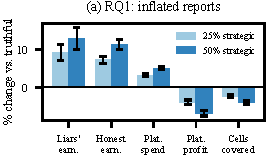
\includegraphics[width=0.245\textwidth]{figs/rq1_lying.pdf}\hfill
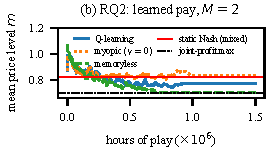
\includegraphics[width=0.245\textwidth]{figs/rq2_qlearning.pdf}\hfill
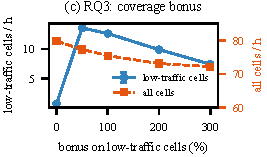
\includegraphics[width=0.245\textwidth]{figs/rq3_bonus.pdf}\hfill
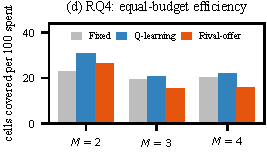
\includegraphics[width=0.245\textwidth]{figs/rq4_methods.pdf}
\caption{(a) Change when 25\% or 50\% of users inflate reports ($M{=}2$, $B{=}300$; mean $\pm$ s.d., 10 seeds). (b) Mean price level while learning vs.\ Nash and joint-profit benchmarks. (c) Coverage against the bonus (25\% of budget reserved). (d) Cells covered per 100 units spent at equal budgets.}
\label{fig:res}
\end{figure*}

\section{Results}
\emph{Equilibrium.} No user could gain by switching in any of 168 hours (Prop.~1).

\emph{RQ1: yes, both rise.} With 50\% liars ($M{=}2$), spending rises 5.1\%, profit falls 6.9\%, and coverage falls 4.0\%; same sign in all 10 seeds and every $M$ (Fig.~\ref{fig:res}a). Honest users gain nearly as much as liars ($+11.3\%$ vs.\ $+12.8\%$): lying is a public good with a weak private incentive ($\delta{=}1$: profit $-9.7\%$).

\emph{RQ2: lower, but not demonstrably collusion.} With $M{=}2$, Q-learners settle at $m{=}0.75$, below the static mixed-Nash level of 0.82, giving a collusion index $\Delta{=}0.58$ (Fig.~\ref{fig:res}b). Memoryless learners cannot punish yet reach the joint-profit price ($\Delta{=}1$): learning, not enforcement, suppresses pay. For $M{=}3,4$, users earn 14--24\% less than with myopic learners. Rival-offer cuts pay for $M{=}2$, raises it for $M{\ge}3$.

\emph{RQ3: yes; a small bonus fixes it.} At a fixed price only 0.7/342 low-traffic cells are covered per hour (80/1368 overall). A $+50\%$ bonus raises this to 13.6 ($18\times$) for a 3\% loss in total coverage; larger bonuses exhaust the reserve sooner (Fig.~\ref{fig:res}c).

\emph{RQ4: Q-learning, at users' expense.} Q-learning covers the most cells per unit spent for every $M$ ($M{=}2$: 31.0 vs.\ 22.7 per 100 at a fixed price; Fig.~\ref{fig:res}d). But users earn 43\% less and the Gini rises from 0.37 to 0.45; rival-offer is least efficient for $M{\ge}3$.

\section{Limitations and Next Steps}
\emph{Limitations:} Spring Festival week; proxy weights; simplified PACMAB; fixed $\delta$.
\emph{Next steps (toward the 7--9 Dec.\ demo):}
\begin{enumerate}\setlength{\itemsep}{0pt}
\item Test RQ1 on PACMAB's actual algorithm; let users learn $\delta$.
\item Design report defences (trimming, capping, spot checks).
\item Add MSensing/deferred acceptance; sensitivity tests.
\end{enumerate}

\begin{thebibliography}{4}
\bibitem{dongare} S.~J. Dongare \emph{et al.}, ``Dynamic hypergame for task assignment in multi-platform mobile crowdsensing under incomplete information,'' arXiv:2605.03569, 2026.
\bibitem{calvano} E.~Calvano, G.~Calzolari, V.~Denicol\`o, and S.~Pastorello, ``Artificial intelligence, algorithmic pricing, and collusion,'' \emph{Amer. Econ. Rev.}, vol.~110, no.~10, 2020.
\bibitem{tdrive} J.~Yuan \emph{et al.}, ``T-Drive: Driving directions based on taxi trajectories,'' in \emph{Proc. ACM SIGSPATIAL GIS}, 2010.
\bibitem{geolife} Y.~Zheng, X.~Xie, and W.-Y. Ma, ``GeoLife: A collaborative social networking service among user, location and trajectory,'' \emph{IEEE Data Eng. Bull.}, 2010.
\end{thebibliography}
\end{document}
